% !TeX document-id = {f19fb972-db1f-447e-9d78-531139c30778}
% !BIB program = biber

%\documentclass[handout]{beamer}
\documentclass[compress]{beamer}
\usepackage[T1]{fontenc}
\usetheme[block=fill,subsectionpage=progressbar,sectionpage=progressbar]{metropolis} 
\usepackage{graphicx}

\usepackage{wasysym}
\usepackage{etoolbox}
\usepackage[utf8]{inputenc}

\usepackage{pifont}

\usepackage{threeparttable}
\usepackage{subcaption}

\usepackage{tikz-qtree}
\usepackage{neuralnetwork}

\setbeamercovered{still covered={\opaqueness<1->{5}},again covered={\opaqueness<1->{100}}}


\usepackage{listings}

\lstset{
	basicstyle=\scriptsize\ttfamily,
	columns=flexible,
	breaklines=true,
	numbers=left,
	%stepsize=1,
	numberstyle=\tiny,
	backgroundcolor=\color[rgb]{0.85,0.90,1}
}



\lstnewenvironment{lstlistingoutput}{\lstset{basicstyle=\footnotesize\ttfamily,
		columns=flexible,
		breaklines=true,
		numbers=left,
		%stepsize=1,
		numberstyle=\tiny,
		backgroundcolor=\color[rgb]{.7,.7,.7}}}{}


\lstnewenvironment{lstlistingoutputtiny}{\lstset{basicstyle=\tiny\ttfamily,
		columns=flexible,
		breaklines=true,
		numbers=left,
		%stepsize=1,
		numberstyle=\tiny,
		backgroundcolor=\color[rgb]{.7,.7,.7}}}{}


% color-coded listings; replace those above 
\usepackage{xcolor}
\usepackage{minted}
\definecolor{listingbg}{rgb}{0.87,0.93,1}
\setminted[python]{
	frame=none,
	framesep=1mm,
	baselinestretch=1,
	bgcolor=listingbg,
	fontsize=\scriptsize,
	linenos,
	breaklines
	}


\usepackage[american]{babel}
\usepackage{csquotes}
\usepackage[style=apa, backend = biber]{biblatex}
\renewcommand*{\bibfont}{\tiny}


\usepackage{tikz}
\usetikzlibrary{shapes,arrows,matrix}
\usepackage{multicol}

\usepackage{subcaption}

\usepackage{booktabs}
\usepackage{graphicx}



\makeatletter
\setbeamertemplate{headline}{%
	\begin{beamercolorbox}[colsep=1.5pt]{upper separation line head}
	\end{beamercolorbox}
	\begin{beamercolorbox}{section in head/foot}
		\vskip2pt\insertnavigation{\paperwidth}\vskip2pt
	\end{beamercolorbox}%
	\begin{beamercolorbox}[colsep=1.5pt]{lower separation line head}
	\end{beamercolorbox}
}
\makeatother





\setbeamercolor{section in head/foot}{fg=normal text.bg, bg=structure.fg}


\newcommand{\instruction}[1]{\emph{\textcolor{gray}{[#1]}}}



\newcommand{\question}[1]{
	\begin{frame}[plain]
	\begin{columns}
		\column{.3\textwidth}
		\makebox[\columnwidth]{
			
\includegraphics[width=\columnwidth,height=\paperheight,keepaspectratio]{mannetje.png}}
		\column{.7\textwidth}
		\large
		\textcolor{orange}{\textbf{\emph{#1}}}
	\end{columns}
\end{frame}}


\tikzstyle{block} = [rectangle, draw, fill=blue!20, 
text width=5em, text centered, rounded corners, minimum height=4em]
\tikzstyle{line} = [draw]
\tikzstyle{pijltje} = [draw, -latex']
\tikzstyle{cloud} = [draw, ellipse,fill=red!20, node distance=3cm,
minimum height=2em, text width=4em, text centered,]


\setbeamercovered{transparent}

\addbibresource{../../resources/literature.bib}
\graphicspath{{../../resources/img/}}


\begin{document}

\title[Big Data and Automated Content Analysis]{\textbf{Big Data and Automated Content Analysis (6EC)} 
\\Week 6: »Unsupervised machine learning«
\\Monday}
\author[Anne Kroon]{Anne Kroon\\ \footnotesize{a.c.kroon@uva.nl, @annekroon \\}}
\date{May 8, 2023}
\institute[UvA CW]{UvA RM Communication Science}


\begin{frame}{}
	\titlepage
\end{frame}

\begin{frame}{Today}
	\tableofcontents
\end{frame}

\question{Everything clear from previous weeks? Questions?}

\begin{frame}[standout]
This week, we will get a general overview of working with textual data. Due to a lack of time, I will introduce you to some of the basic concepts, point you to resources, and give you a practical, hands-on introduction. 
\end{frame}

\begin{frame}{\cite{Boumans2016}: Types of Automated Content Analysis}
	\makebox[\columnwidth]{	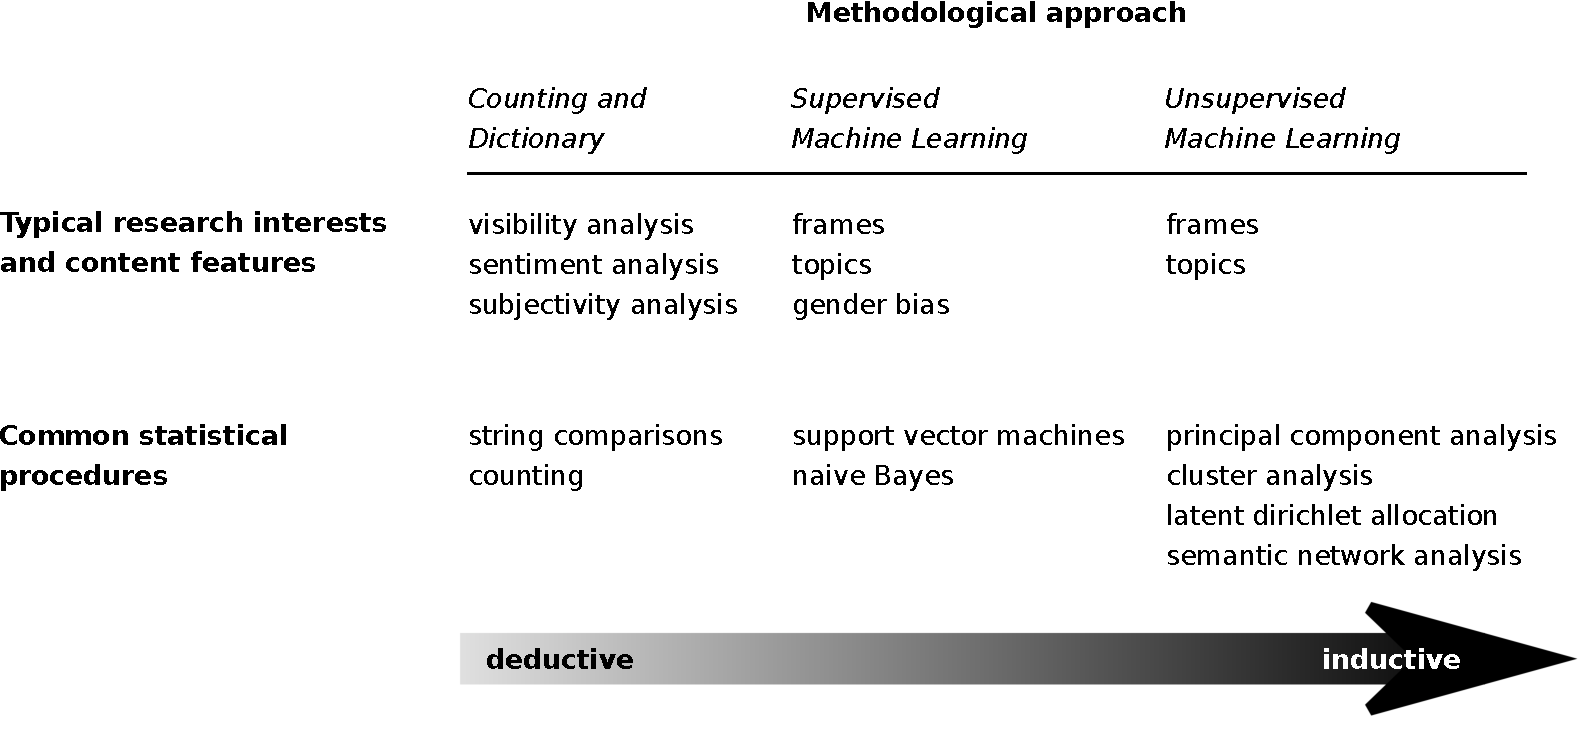
\includegraphics[width=\columnwidth,height=.8\paperheight,keepaspectratio]{boumanstrilling2016}}
\end{frame}

\begin{frame}{Bottom-up vs. top-down}
\begin{block}{Bottom-up}
	\begin{itemize}
		\item Count most frequently occurring words 
		\item Maybe better: Count combinations of words $\Rightarrow$ Which words co-occur together?
	\end{itemize}
	We \emph{don't} specify what to look for in advance	
\end{block}

\onslide<2>{
	\begin{block}{Top-down}
		\begin{itemize}
			\item Count frequencies of pre-defined words
			\item Maybe better: patterns instead of words
		\end{itemize}
		We \emph{do} specify what to look for in advance	
	\end{block}
}

\end{frame}

\begin{frame}[fragile]{A simple bottom-up approach}

\begin{minted}[%
	breaklines,
	linenos,
	fontsize=\scriptsize,
	frame=single,
	xleftmargin=0pt,]
	{python}
from collections import Counter
texts = ["Communication in the Digital Society is a very very complex phenomenon", "I like to study it"]
bottom_up = []
for t in texts:
    bottom_up.append(Counter(t.lower().split()).most_common(3))
    print(bottom_up)
\end{minted}
\pause
This results in:
\begin{minted}[fontsize=\scriptsize]{python}
[('very', 2), ('Communication', 1), ('in', 1)]
[('I', 1), ('like', 1), ('to', 1)]
\end{minted}
\textcolor{red}{\footnotesize{\emph{Please note that you can also write this like:}}}
\pause
\begin{minted}[%
	breaklines,
	linenos,
	fontsize=\scriptsize,
	frame=single,
	xleftmargin=0pt,]
	{python}
bottom_up = [Counter(t.split()).most_common(3) for t  in texts]
\end{minted}
\begin{itemize}
	\tiny{
		\item This is \emph{exactly} the same, just shorter (and faster). 
		\item You do \emph{not} have to use list comprehensions, but it helps if you can read them. }
\end{itemize}

\end{frame}

\begin{frame}[fragile]{A simple top-down approach}
\begin{minted}[%
	breaklines,
	linenos,
	fontsize=\scriptsize,
	frame=single,
	xleftmargin=0pt,]
	{python}
texts = ["Communication in the Digital Society is a very very complex phenomenon", "I like to study it"]
features = ["communication", "digital", "study"]
for t in texts:
    print(f"\nAnalyzing '{t}':")
    for f in features:
        print(f"{f} occurs {t.lower().count(f)} times")
\end{minted}
\pause
\begin{minted}[fontsize=\tiny]{python}
Analyzing 'Communication in the Digital Society is a very very complex phenomenon':
communication occurs 1 times
digital occurs 1 times
study occurs 0 times
	
Analyzing 'I like to study it':
communication occurs 0 times
digital occurs 0 times
study occurs 1 times	
\end{minted}
\end{frame}

\question{When would you use which approach?}

\begin{frame}{Some considerations}
\begin{itemize}[<+->]
	\item Both can have a place in your workflow (e.g., bottom-up as first exploratory step)
	\item You have a clear theoretical expectation? Bottom-up makes little sense.
	\item But in any case: you need to transform your text into something ``countable''.
\end{itemize}
\end{frame}

\section{Unsupervised Machine Learning for Text Classification}


\begin{frame}{Supervised vs Unsupervised}
	\begin{columns}[t]
		\column{.5\textwidth}
		
		\begin{block}<1-4>{Supervised machine learning}
			You have a dataset with both predictor and outcome (independent and dependent variables; features and labels) --- a \emph{labeled} dataset.
			\onslide<2>{
				\footnotesize{Think of regression: You measured \texttt{x1}, \texttt{x2}, \texttt{x3} and you want to predict \texttt{y}, which you also measured}}
		\end{block}
		
		\column{.5\textwidth}
		
		\begin{block}<3->{Unsupervised machine learning}
			You have no labels. \onslide<4>{(\footnotesize{You did not measure \texttt{y})}}\\
			\onslide<5>{\textbf{You might already know \emph{some} techniques to figure out whether \texttt{x1}, \texttt{x2},\ldots \texttt{x\_i} co-occur} \begin{itemize}
					\item Principal Component Analysis (PCA) and Singular Value Decomposition (SVD)
					\item Cluster analysis
					\item Topic modelling (Non-negative matrix factorization and Latent Dirichlet Allocation)
					\item \ldots
			\end{itemize}}
		\end{block}
		
	\end{columns}
	
\end{frame}

\subsection{An introduction to LDA}

\begin{frame}{}
	Enter \textbf{topic modeling with Latent Dirichlet Allocation (LDA)}
\end{frame}


\begin{frame}{LDA, what's that?}
	\begin{block}{No mathematical details here, but the general idea}
		\begin{itemize}
			\item There are $k$ topics, $T_1$\ldots$T_k$
			\item Each document $D_i$ consists of a mixture of these topics, e.g.$80\% T_1, 15\% T_2, 0\% T_3, \ldots 5\% T_k $
			\item On the next level, each topic consists of a specific probability distribution of words
			\item Thus, based on the frequencies of words in $D_i$, one can infer its distribution of topics
			\item Note that LDA is a Bag-of-Words (BOW) approach
		\end{itemize}
	\end{block}
	
\end{frame}


\begin{frame}[fragile]{Doing a LDA in Python}
	We will use gensim \parencite{Rehurek10softwareframework} for this (make sure you have version >4.0)
	
	Let us assume you have a list of lists of documents called \texttt{texts}:
	\begin{minted}[%
		breaklines,
		linenos,
		fontsize=\tiny,
		frame=single,
		xleftmargin=0pt,]
		{python}
print(texts[0][:115])
	\end{minted}
	\pause
	which looks something like:
	\begin{minted}[%
		fontsize=\tiny,
		breaklines,]
		{python}
'Stop the presses: CNN covered some actual news yesterday when it reported on the story of medical kidnapping victim Alyssa Gilderhus at the Mayo Clinic. But was it actually InfoWars and FreeMartyG which publicly shamed CNN into doing this real journalism? Cue the Mission Impossible theme music for this one...\n\nThis mission, as we accepted it, began more than a year ago during the baby Charlie Gard medical kidnapping scandal in the UK and we thought that it had ended with an apparently unsuccessf'
	\end{minted}
	
	\tiny{{\v R}eh{\r u}{\v r}ek, R., \& Sojka, P. (2010). Software framework for topic modelling with large corpora. \emph{Proceedings of the LREC 2010 Workshop on New Challenges for NLP Frameworks}, pp. 45–50. Valletta, Malta: ELRA. }
\end{frame}

\begin{frame}[fragile]{Preprocessing}
	Your preprocessing steps and feature engineering decisions \emph{largely} affect your topics
	\begin{enumerate}
		\item<1-> You can apply 'manual' preprocessing steps \dots
		\item<2->\dots In isolation or combination with for example \texttt{tfidf} transformations
	\end{enumerate}
	\pause
	\pause
	\begin{minted}[%
		breaklines,
		linenos,
		fontsize=\tiny,
		frame=single,
		xleftmargin=0pt,]
		{python}
texts_clean = [text.lower() for text in texts]
texts_clean=[" ".join(text.split()) for text in texts_clean]  #remove dubble spaces
texts_clean = ["".join([l for l in text if l not in punctuation]) for text in texts_clean] #remove punctuaction
texts_clean[0][:500]
	\end{minted}
	\pause
	which looks something like:
	\begin{minted}[%
		breaklines,
		fontsize=\tiny,]
		{python}
'stop the presses cnn covered some actual news yesterday when it reported on the story of medical kidnapping victim alyssa gilderhus at the mayo clinic but was it actually infowars and freemartyg which publicly shamed cnn into doing this real journalism cue the mission impossible theme music for this one this mission as we accepted it began more than a year ago during the baby charlie gard medical kidnapping scandal in the uk and we thought that it had ended with an apparently unsuccessful april '
	\end{minted}
\end{frame}

\begin{frame}[fragile]{Preprocessing}
	Without \emph{stopword removal},  \emph{tfidf} transformation and/or \emph{pruning}, you topics will not be very informative.
	\pause
	\begin{minted}[%
		breaklines,
		linenos,
		fontsize=\tiny,
		frame=single,
		xleftmargin=0pt,]
		{python}
mystopwords = set(stopwords.words('english')) # use default NLTK stopword list; alternatively:
# mystopwords = set(open('mystopwordfile.txt').readlines())  #read stopword list from a textfile with one stopword per line
texts_clean = [" ".join(word for word in text.split() if word not in mystopwords) for text in texts_clean]
texts_clean[0][:500]
	\end{minted}
	\pause
	which looks something like:
	\begin{minted}[%
		breaklines,
		fontsize=\tiny,]
		{python}
'stop presses cnn covered actual news yesterday reported story medical kidnapping victim alyssa gilderhus mayo clinic actually infowars freemartyg publicly shamed cnn real journalism cue mission impossible theme music one mission accepted began year ago baby charlie gard medical kidnapping scandal uk thought ended apparently unsuccessful april fools joke cnn sure many recall charlie gard infant rare form otherwise notsorare condition mitochondrial disease story went viral made international news '
	\end{minted}
\end{frame}

\begin{frame}[fragile]{Tokenization}
	\texttt{gensim} expects a list of words (hence: \texttt{tokenize} your corpus)
	\pause
	\begin{minted}[%
		breaklines,
		linenos,
		fontsize=\tiny,
		frame=single,
		xleftmargin=0pt,]
		{python}
tokenized_texts_clean = [TreebankWordTokenizer().tokenize(text) for text in texts_clean ] # tokenize texts; convert all strings to a list of tokens
tokenized_texts_clean[0][:500]
	\end{minted}
	\pause
	which looks something like:
	\begin{minted}[%
		breaklines,
		fontsize=\tiny,]
		{python}
['stop',
'presses',
'cnn',
'covered',
'actual',
'news',
'yesterday',
'reported',
'story',
..
	\end{minted}
\end{frame}

\begin{frame}[fragile]{LDA implementation}
	\texttt{LDA} implementation
	\pause
	\begin{minted}[%
		breaklines,
		linenos,
		fontsize=\tiny,
		frame=single,
		xleftmargin=0pt,]
		{python}
raw_m1 = tokenized_texts_clean
		
# assign a token_id to each word
id2word_m1 = corpora.Dictionary(raw_m1)   
# represent each text by (token_id, token_count) tuples
ldacorpus_m1 = [id2word_m1.doc2bow(text) for text in raw_m1] 
		
#estimate the model
lda_m1 = models.LdaModel(ldacorpus_m1, id2word=id2word_m1, num_topics=10)
lda_m1.print_topics()
	\end{minted}
	\pause
	
	\begin{minted}[%
		breaklines,
		fontsize=\tiny,]
		{python}
[(0, '0.015*"trump" + 0.012*"said" + 0.006*"president" + 0.006*"people" + 0.004*"cnn" + 0.004*"us" + 0.004*"house" + 0.004*"news" + 0.003*"also" + 0.003*"twitter"'),
(1,'0.010*"said" + 0.008*"trump" + 0.004*"one" + 0.004*"people" + 0.004*"us" + 0.004*"president" + 0.004*"would" + 0.003*"media" + 0.003*"also" + 0.003*"new"'),
(2, '0.011*"trump" + 0.009*"said" + 0.007*"president" + 0.005*"would" + 0.004*"people" + 0.004*"us" + 0.003*"also" + 0.003*"like" + 0.003*"news" + 0.003*"state"'),
(3, '0.010*"trump" + 0.006*"president" + 0.005*"said" + 0.004*"would" + 0.004*"us" + 0.003*"also" + 0.003*"people" + 0.003*"media" + 0.003*"news" + 0.003*"one"'),
	\end{minted}
\end{frame}


\begin{frame}[fragile]{Visualization with pyldavis}
	\begin{minted}[%
		breaklines,
		linenos,
		fontsize=\tiny,
		frame=single,
		xleftmargin=0pt,]
		{python}
import pyLDAvis
import pyLDAvis.gensim_models as gensimvis
# first estiate gensim model, then:
vis_data = gensimvis.prepare(lda_m1,ldacorpus_m1,id2word_m1)
pyLDAvis.display(vis_data)
	\end{minted}
	\makebox[\linewidth]{
		\includegraphics[width=\paperwidth,height=.5\paperheight,keepaspectratio]{../pictures/lda}}
\end{frame}

\iffalse
\begin{frame}{Visualization with pyldavis}
	Short note about the $\lambda$ setting:
	
	It influences the ordering of the words in pyldavis.
	
	\begin{quote}
		``For $\lambda = 1$, the ordering of the top words is equal to the ordering of the standard conditional word probabilities. For $\lambda$ close to zero, the most specific words of the topic will lead the list of top words. In their case study, Sievert and Shirley (2014, p. 67) found the best interpretability of topics using a  $\lambda$-value close to .6, which we adopted for our own case'' (Maier et al., 2018, p.~107)
	\end{quote}
	
	
	\tiny{Maier, D., Waldherr, A., Miltner, P., Wiedemann, G., Niekler, A., Keinert, A., \ldots Adam, S. (2018). Applying LDA Topic Modeling in Communication Research: Toward a Valid and Reliable Methodology. \textit{Communication Methods and Measures, 12}(2--3), 93--118. doi:10.1080/19312458.2018.1430754}
\end{frame}
\fi


\subsection{Choosing the best (or a good) topic model}

\begin{frame}{Choosing the best (or a good) topic model}
	\begin{itemize}
		\item There is no single best solution (e.g., do you want more coarse of fine-grained topics?)
		\item Non-deterministic
		\item Very sensitive to preprocessing choices
		\item Interplay of both metrics and (qualitative) interpretability 
	\end{itemize}
	
	See for more elaborate guidance:
	
	\tiny{Maier, D., Waldherr, A., Miltner, P., Wiedemann, G., Niekler, A., Keinert, A., \ldots Adam, S. (2018). Applying LDA Topic Modeling in Communication Research: Toward a Valid and Reliable Methodology. \textit{Communication Methods and Measures, 12}(2--3), 93--118. doi:10.1080/19312458.2018.1430754}
	
\end{frame}



\begin{frame}{Evaluation metrics}
	\begin{block}{Qualitative: human judgement}
		Observation and interpretation based: observe the top N words in your topic, and evaluate the quality of the coherence of the topic.  Can you identify words that do not belong to a topic?
	\end{block}
	
	\pause 
	\begin{block}{Quantitative: coherence}
		\begin{itemize}
			\item mean coherence of the whole model: attempts to quantify the interpretability
			\item coherence per topic: allows to get topics that are most likely to be coherently interpreted (\texttt{.top\_topics()})
		\end{itemize}
	\end{block}
	
\end{frame}


\begin{frame}{So, how do we do this?}
	\begin{itemize}[<+->]
		\item Estimate multiple models, store the metrics for each model, and then compare them (numerically, or by plotting)
		\item Idea: We select some candidate models, and then look whether they can be interpreted.
		\item But what can we tune?
	\end{itemize}
\end{frame}


\begin{frame}{Choosing $k$: How many topics do we want?}
	\begin{itemize}
		\item Typical values: $10<k<200$
		\item Too low: losing nuance, so broad it becomes meaningless
		\item Too high: picks up tiny pecularities instead of finding general patterns
		\item There is no inherent ordering of topics
		\item We can throw away or merge topics later, so if out of $k=50$ topics 5 are not interpretable and a couple of others overlap, it still may be a good model
	\end{itemize}
\end{frame}


\begin{frame}[fragile]{Choosing $\alpha$: how sparse should the document-topic distribution $\theta$ be?}
	\begin{itemize}
		\item The higher $\alpha$, the more topics per document 
		\item Default: $1/k$
		\item But: We can explicitly change it, or -- really cool -- even learn $\alpha$ from the data (\texttt{alpha = "auto"})
	\end{itemize}
	
	\pause 
	

	\begin{minted}[%
		breaklines,
		linenos,
		fontsize=\tiny,
		frame=single,
		xleftmargin=0pt,]
		{python}
mylda =LdaModel(corpus=tfidfcorpus[ldacorpus], id2word=id2word, num_topics=50, alpha='auto', passes=10)
	\end{minted}
	
\end{frame}


\iffalse
\begin{frame}{Choosing $\eta$: how sparse should the topic-word distribution $\lambda$ be?}
	\begin{itemize}
		\item Can be used to boost specific words
		\item Can also be learned from the data 
	\end{itemize}
	
	\pause
Takeaway: Even though you can do \texttt{eta="auto"}, this usually does not help you much.
	
\end{frame}
Takeaway: It takes longer, but you probably want to learn alpha from the data, using multiple passes:
\fi

% \subsection{Drawbacks of LDA topic models}


\subsection{Using topic models}

\begin{frame}{Using topic models}
	
You got your model -- what now?
	
	\begin{enumerate}
		\item Assign topic scores to documents
		\item Label topics
		\item Merge topics, throw away boilerplate topics and similar (manually, or aided by cluster analysis)
		\item Compare topics between, e.g., outlets
		\item or do some time-series analysis.
	\end{enumerate}
	
	
	Example:
	\tiny{Tsur, O., Calacci, D., \& Lazer, D. (2015). A Frame of Mind: Using Statistical Models for Detection of Framing and Agenda Setting Campaigns. \textit{Proceedings of the 53rd Annual Meeting of the Association for Computational Linguistics and the 7th International Joint Conference on Natural Language Processing} (pp. 1629–1638).}
	
\end{frame}



\question{Any questions?}

\section{Next steps}

\begin{frame}[standout]
Take-home exam: you have time until Thursday 11th, end of the day

An example notebook with code for running LDA models can be found here:
\large{\url{https://github.com/uvacw/teaching-bdaca/blob/main/6ec-course/week06/exercises/}}
\end{frame}



\begin{frame}[allowframebreaks,plain]
	\printbibliography
\end{frame}



\end{document}
